% mainfile: ../../../../master.tex
\subsection{Nucleic acids quantification with NanoDrop\cR ND-1000 Spectrophotometer}
% The part of the label after the colon must match the file name. Otherwise,
% conditional compilation based on task labels does NOT work.
\label{task:20180213_cj2}
\tags{lab,dna,rna,qnt}
\authors{cj}
%\files{}
%\persons{}

Defrost samples on ice:
\begin{itemize}
\item \texttt{CJ20180213\_DNA\_AllPrep} (DNA was eluted with a total of 150~\uL Tris-HCl ph 8)
\item \texttt{CJ20180213\_RNA\_AllPrep} (RNA was eluted with a total of 80~\uL RNase-free water from the kit)
\end{itemize}

The blank for the DNA concentration measurment was done with the same Tris-HCl buffer pH 8. The blank for the RNA concentration measurement was done with sterile MilliQ water (because it was too risky to open the RNase-free water there).

\begin{figure}[H] % position of the figure 
    \centering
    \caption{Screen captures of the NanoDrop\cR analysis}
    \label{fig:CJ20180213_DNA_RNA_AllPrep}
    \begin{subfigure}[b]{0.49\textwidth}
        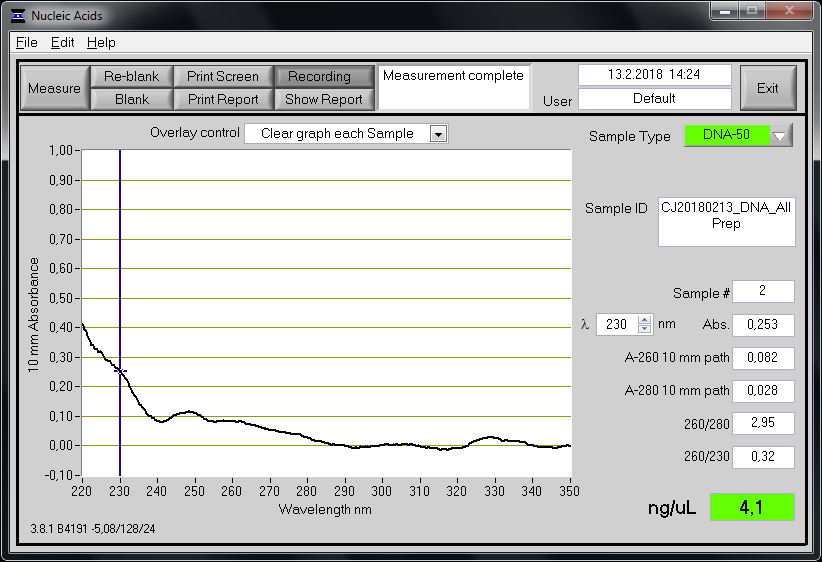
\includegraphics[width=\textwidth]{graphics/screenshots/CJ20180213_DNA_AllPrep.png}
        \caption{DNA}
        \label{sfig:CJ20180213_DNA_AllPrep}
    \end{subfigure}
    ~ 
    \begin{subfigure}[b]{0.49\textwidth}
        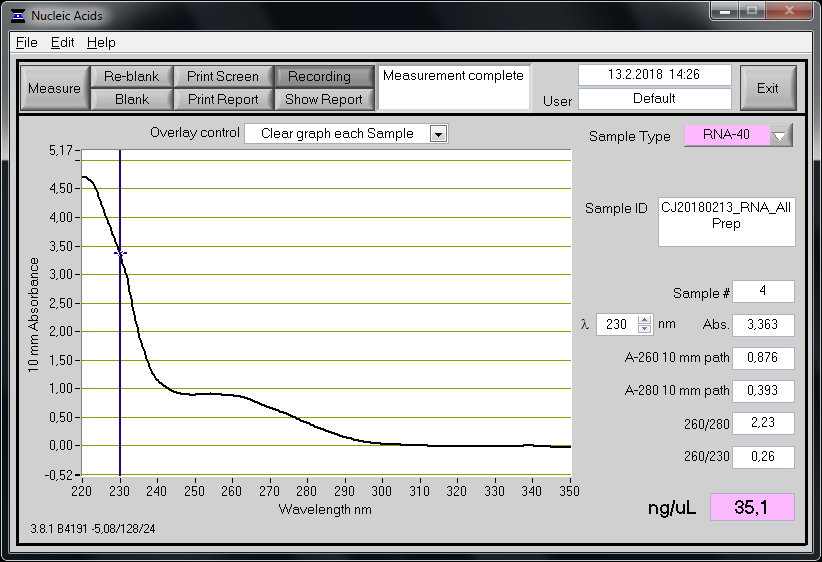
\includegraphics[width=\textwidth]{graphics/screenshots/CJ20180213_RNA_AllPrep.png}
        \caption{RNA}
        \label{sfig:CJ20180213_RNA_AllPrep}
    \end{subfigure}
\end{figure}

\begin{table}[htbp]
\caption{res/nanodrop/CJ20180213.txt}
\label{tab:CJ20180213_nanodrop}
\centering
\begin{tabular}{l l l l l l l l l l l l l }
\toprule
Sample ID & Time  & ng/ul  & A260  & A280  & 260/280  & 260/230  \\ \midrule
\texttt{CJ20180213\_BLANK} & 14:22 & -1,94 & -0,039 & -0,029 & 1,32 & 1,13 \\
\texttt{CJ20180213\_DNA\_AllPrep} & 14:23 & 4,11 & 0,082 & 0,028 & 2,95 & 0,32 \\
\texttt{CJ20180213\_BLANK} & 14:25 & 0,42 & 0,010 & -0,000 & -35,25 & 1,95 \\
\texttt{CJ20180213\_RNA\_AllPrep} & 14:26 & 35,06 & 0,876 & 0,393 & 2,23 & 0,26 \\
\bottomrule
\end{tabular}
\\
User: Default - Date: 13.2.2018 - Constant: 40,00 - Cursor position: 230 \
\end{table}

\sidenote{Nucleotides, RNA, ssDNA, and dsDNA all will absorb at 260 nm and contribute to the total absorbance.}

The expected value for the 260/280 ratio is approx. 1.8 for "pure DNA". The 260/280 value for my DNA sample is 2.95 which is a lot higher than the expected value. It is known that small changes in the pH of the solution will cause the 260/280 to vary \citep{mackey1997effect}. Acidic solutions will under-represent the 260/280 ratio by 0.2- 0.3, while a basic solution will over-represent the ratio by 0.2-0.3. The buffer is slighly alkaline (pH 8) which is likely to over-represent the 260/280 ratio ... but here it is a lot higher. 

Abnormal 260/280 ratios usually indicate that a sample is contaminated by residual phenol, guanidine, or other reagent used in the extraction protocol, in which case the ratio is normally low which is not the case here (I did not use any of these reagents). Inaccurate ratios may also be encountered at very low concentrations (<10 ng /\uL) of nucleic acids. High 260/280 purity ratios are not necessarily indicative of a problem. However, a very high ratio can suggest a poor quality blank eliminating too much signal near the 280 nm wavelength. Moreover, the spectrum obtained for the DNA (see fig \ref{sfig:CJ20180213_DNA_AllPrep}) does not even show a clear peak for DNA.


